Ein homogenes Brett (Länge \LBO, Masse \mBO) trägt an seinem rechten Ende ein kleines Bleistück von \mPbO. Es ist um eine waagrechte, reibungsfreie Achse D drehbar, die durch die Mitte des Bretts geht.
\begin{center}
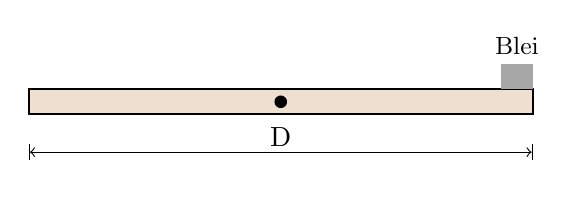
\begin{tikzpicture}[scale=0.8]
 \fill[brown!25] (-4,-0.2) rectangle (4,0.2);
 \draw[thick] (-4,-0.2) rectangle (4,0.2);
 \fill[gray!70] (3.5,0.2) rectangle (4,0.6);
 \node[above] at (3.75,0.6) {\small Blei};
 \fill (0,0) circle (0.1);
 \node[below] at (0,-0.25) {D};
 \draw[|<->|] (-4,-0.8) -- (4,-0.8) node[midway, below] {\LBO};
\end{tikzpicture}
\end{center}
Ein Schüler schreibt:

\begin{quote}
Die Achse geht durch die Mitte des Bretts, also hat die Gewichtskraft keinen Hebelarm. Das Brett ist im indifferenten Gleichgewicht: Es bleibt in jeder Lage stehen, auch waagrecht.
\end{quote}

\begin{abcliste}
\abc
Was ist an dieser Überlegung falsch?

\abc
Wie weit von der Achse entfernt liegt der Schwerpunkt S des Bretts mit dem Blei? \DuSie{Betrachte}{Betrachten Sie} das Blei als punktförmig.

\abc
Wie gross ist das Drehmoment der Gewichtskraft bezüglich D, wenn man das Brett waagrecht hält?

\abc
In welcher Lage kommt das Brett (mit etwas Reibung in der Achse) zur Ruhe? Welche Art von Gleichgewicht ist das? Gibt es eine weitere Gleichgewichtslage?
\end{abcliste}
